\documentclass{article}
\usepackage{graphicx} % Required for inserting images
\usepackage{pgf}
\usepackage{lmodern}
\usepackage{import}
\usepackage{booktabs}
\usepackage{tabu}
\usepackage{float}
\usepackage[hidelinks]{hyperref}
\usepackage{amsmath}
\usepackage[margin=1in]{geometry}

\setlength{\parskip}{1em}
\setlength{\parindent}{0em}

\title{GYRO REPORT}
\author{Toby Nguyen - z5416116}
\date{May 2024}

\begin{document}
\begin{center}
    \huge{Gyroscopes} \\[10pt]
    \large{Toby Nguyen - z5416116}
\end{center}
\tableofcontents
\newpage

\section{Introduction}
In rotational mechanics, there are phenomena analog to translational mechanics
such as momentum of inertia, torque and angular velocity, acceleration and
momentum. However, certain phenomena in rotational mechanics such as precession
and nutation do not have such analogs and are thus inherently unintuitive. To 
explore these mechanics and to build the intuition, a mathematical derivation is required. 

\subsection{Precession}
Precession is the motion where the spinning object rotations about a vertical axis, 
in addition to the rotation about its own axis.

In its inertial reference frame, the total torque of a spinning object is related to its angular momentum,
\begin{equation}
    \vec{\tau} = \frac{d\vec{L}}{dt}.
\end{equation}

However from a fixed reference frame, there must be a second term that accounts 
for the rotation of the inertial reference frame, i.e
\begin{equation}
    \vec{\tau} = \frac{d\vec{L}}{dt} + \vec{\omega} \times \vec{L}.
\end{equation}

This second term suggests that there is a torque that acts perpendicular to
the angular momentum and velocity of the spiining object. 
\begin{equation}
    \vec{\tau}_p = \vec{\omega}_p \times \vec{L}_s.
\end{equation}

\subsection{Nutation}
Nutation refers to the oscillating motion of a spinning object's own axis with respect
to its original axis' position. Nutation occurs when a transient force acts on the 
spinning object in any direction perpendicular to its angular momentum. Hence,
\begin{equation}
    \vec{\tau}_n = \vec{\omega}_n \times \vec{L}_s.
\end{equation}

\section{Aim}
To investigate the rotational mechanics phenomena of  moment of inertia, 
angular momentum and velocity and precession and nutation. 
Ultimately, to verify Equation (3) and provide some insights 
into Eqn (4).
\section{Method}
\subsection{Experimental Setup}
To measure the moment of inertia of the disk, the gyroscope was kept fixed,
only allowed to spin along the axis of the arm. Otherwise, the gyroscope
arm was free and allowed the disk to precess and undergo nutation. Throughout both 
experiments, a bunch of constants were used shown in the Table \ref{fig:table} 
below. The distance from the mass to the fulcrum is denoted by $x$. The radius 
of the disk is denoted by R and the radius of the small disk is denoted by r. 
The mass of the disk is denoted by M.

\begin{table}[H]
    \centering
    \begin{tabular}{c|c}
        Constant & Measurement \\
        \hline
        M & 1.336 $\pm$ 0.0005 kg \\
        R & 0.1225 $\pm$ 0.0005m \\
        r & 0.025 $\pm$ 0.0005m \\
        x & 0.275 $\pm$ 0.0005m 
    \end{tabular}
    \caption{Table displaying measured constants in the experiment}
    \label{fig:table}
\end{table}

\subsubsection{Locked Gyroscope}
Firstly, the gyroscope arm was fixed as shown in Figure \ref{fig:locked} and a mass was 
attached to the cord. The string was wound around the small disk attached to the big disk 
so that the mass carrier, carrying mass 150g, would fall from a desired height, h. The full 
extension of the string was measured to be 58cm and so the mass was released from heights 
8cm, 18cm, 28cm, 38cm and 48cm to measure the height fell by 0.1m, 0.2m, 0.3m, 0.4m and 
0.5m. The time it took to  fall was recorded on a stopwatch which began as the mass carrier 
was released and stopped when the string was at its full extension.
\begin{figure}[H]
    \centering
    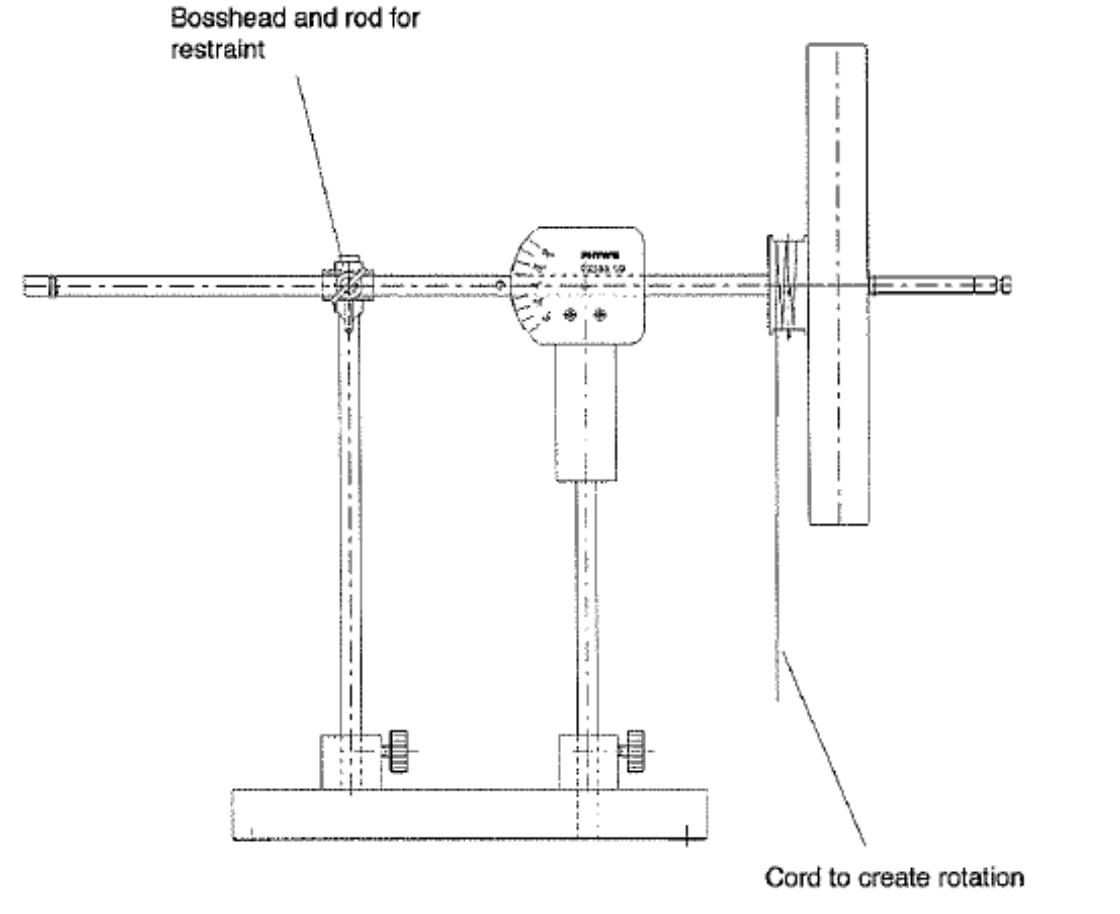
\includegraphics[width=0.5\textwidth]{figure1.png}
    \caption{Diagram of the locked configuration of the gyroscope.}
    \label{fig:locked}
\end{figure}
In this situation, the force on the mass downwards is driven by the difference
between the acceleration due to gravity downwards and the acceleration due to the tension
in the string upwards multiplied by the mass of the object,
\begin{equation}
     F = m(g-a).
\end{equation}
The acceleration due to the tension in the string is related to the angular 
acceleration of the small disk. This is because as the string's 
tensions increases, it will push the small disk, causing an 
angular acceleration.

\begin{equation}
    a = r\alpha.
\end{equation}

The angular acceleration of the small disk can be assumed to be the same as 
the angular acceleration of the bigger disk which is related to its moment 
of inertia. (The angle of the incoming force is $90^{\circ}$).

\begin{equation}
    \alpha = \frac{rF}{I_s}.
\end{equation}

Combining Eqns. (6) and (7) gives,
\begin{equation}
    \begin{split}
    a = \frac{r^2m(g-a)}{I_s} \\
    = \frac{r^2mg-r^2ma}{I_s} \\
    aI_s+r^2ma = mgr^2 \\
    a = \frac{mgr^2}{I_s+mr^2}  
    \end{split}
\end{equation}

Using kinematic equations, the acceleration of the mass is related 
to the height and time to fall,
\begin{equation}
    \begin{split}
        h  = \frac{1}{2}at^2_F \\
        a = \frac{2h}{t^2_F} 
    \end{split}
\end{equation}

Combining Eqns. (8) and (9) gives,

\begin{equation}
    \begin{split}
        \frac{2h}{t^2_F} = \frac{mgr^2}{I_s+mr^2} \\
        t^2_F = \frac{2I_s+2mr^2}{mgr^2}h    
    \end{split}
\end{equation}

\subsubsection{Free Gyroscope}
To measure the angular velocity of precession and nutation, the support beam 
was removed and the gyroscope arm was allowed to move freely, shown in Figure \ref{fig:free}. 
The procedure for the measurement of precession and the measurement of nutation with 
precession was the same whereas the measurement of nutation without precession was differed
slightly.

\begin{figure}[H]
    \centering
    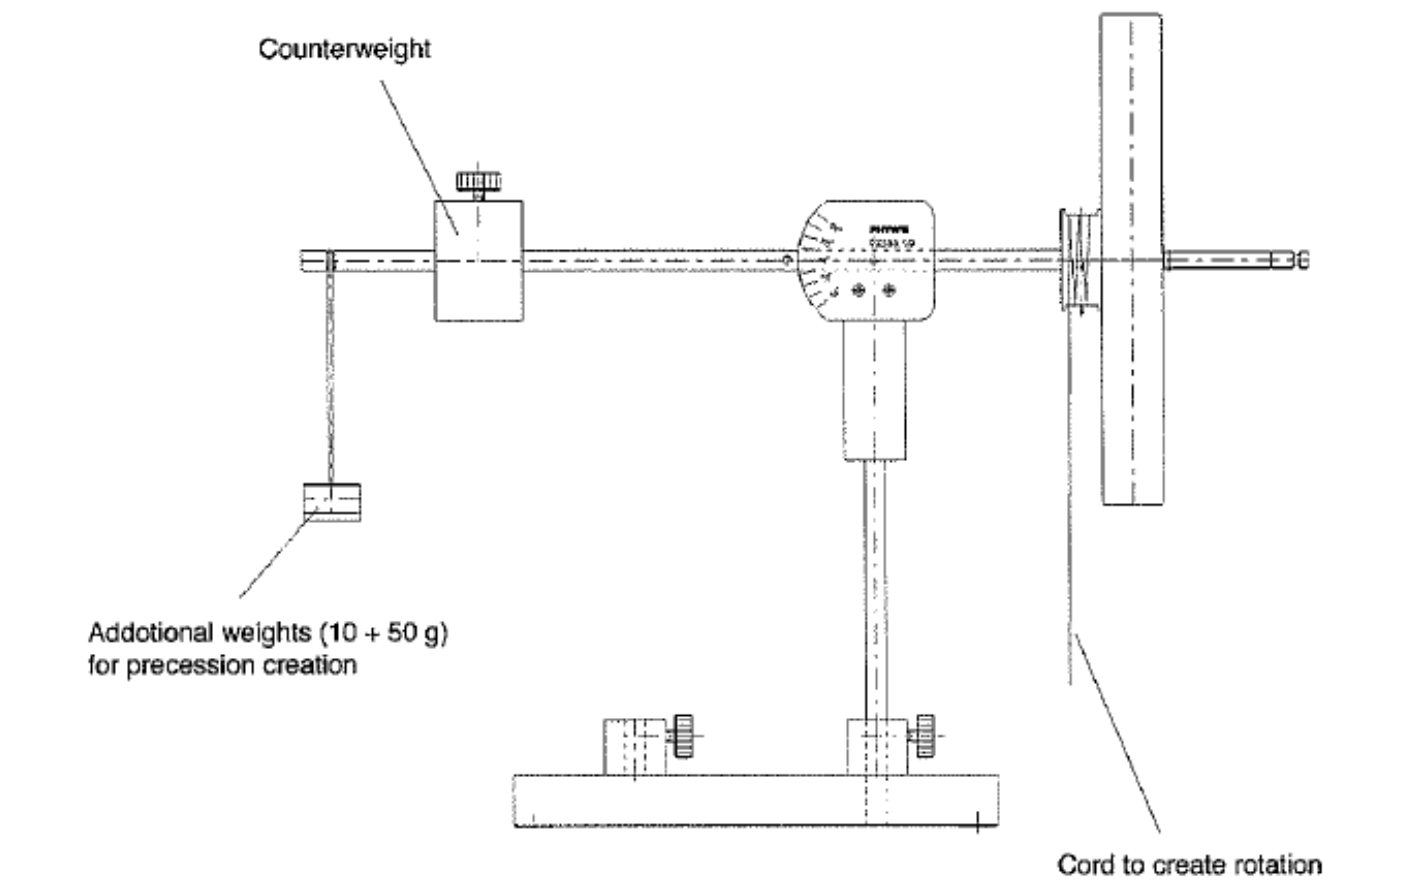
\includegraphics[width=0.5\textwidth]{figure2.png}
    \caption{Diagram of free configuration of the gyroscope.}
    \label{fig:free}
\end{figure}

In all three measurements, the angular velocity of the spinning disk was calculated by
using an optical gate counter, counting the amount of revolutions, n, in 10 seconds.
To account for frictional effects on the spinning disk, two counts were done, one before
the precession or nutation and one after and the average of the two counts was used,
\begin{equation}
    \omega_s = \frac{2\pi n_{avg}}{10}.
\end{equation}

For precession without nutation, the disk was spun by pulling the cord and its angular
velocity of spin was initially measured. A mass carrier containing weights of 20g, 40g,
60g, 90g and 140g, combining for a total mass of 30g, 50g, 70g, 100g and 150g was added
to the opposite end of the gyroscope arm as displayed in Figure \ref{fig:free}. The spinning
disk now began to precess and its half period was recorded in order to calculate its angular
velocity of precession,
\begin{equation}
    \omega_p = \frac{2\pi}{0.5T}.
\end{equation}

With 
reference to Figure \ref{fig:free}, this added mass creates a torque acting into the page
as now there was a force due to gravity acting on the left side of the arm. When the mass
was added, the gyroscope arm began to tilt some degrees, the reason for the volatility of
the tilt can be attributed to the external force from placing down the mass but should be 
explored in further experiments to accurately determine what caused the tilt. Nevertheless,
the angle of tilt, $\theta$, was measured using a protractor attached onto the 
gyroscope arm and the torque due to the added weight can be calculated,

\begin{equation}
    \tau_{mass} = mgx\sin{\theta}.
\end{equation}

The total torque of the gyroscope can be related to its angular momentum,
\begin{equation}
    \vec{\tau} = \frac{\Delta \vec{L}}{\Delta t}.
\end{equation}

From Figure \ref{fig:free}, it can be seen that the direction of torque, into the page, is
perpendicular to the direction of angular momentum. This means that the total torque will 
only change the direction of angular momentum, not its magnitude and so Eqn. (13) can be 
modified,

\begin{equation}
    \vec{\tau} = \frac{\vec{L}\Delta \phi}{\Delta t}
\end{equation}
where $\phi$ is the horizontal angle that angular momentum makes with its vertical axis. 
Therefore the $\frac{\Delta \phi}{\Delta t}$ can be replaced with $\omega_p$ where p denotes 
the motion of precession.

\begin{equation}
    \vec{\tau} = \vec{\omega}_p \times \vec{L}_s.
\end{equation}

This is the same as Eqn. (3) so the 'total torque' in this situation will be just the 
torque due to precession, $\omega_p$. This is because Eqn. (13) should have included 
a change in angular momentum due to the torque created by an unstable centre of mass
however $L_s >> L_{CM}$ so this can be ignored experimentally. 

As $\omega_p$ and $\vec{L}_s$ are perpendicular and $L_s$ can be rewritten as the product
of its angular velocity and momentum of inerita,
\begin{equation}
    \begin{split}
    \tau_p &= |\omega_p||L_s| \\
    &= \omega_p I_s \omega_s   
    \end{split}
\end{equation} 

Rearranging and substituting in Eqn. (12),

\begin{equation}
    \omega_p = \frac{gx}{I_s\omega_s}m.
\end{equation}

For measuring nutation with precession, the same method was done except as the mass was
added on, a small knock was also conducted to provide a transient force perpendicular to
the angular momentum. The purpose of this was not to measure the oscillating motion of 
nutation but compare the two motions of precession, one with nutation and one without.

For measuring nutation without precession, the disk was spun on its axis shown in 
Figure \ref{fig:free}. The angular velocity was measured and then varying sized knocks were stuck 
on the end of the gyroscope arm opposite the disk. These knocks were best kept controlled 
by using one finger for 'soft' knock, two fingers for 'medium' knock and three fingers 
for 'hard' knock. As the disk underwent nutation, its number of oscillations, n, were counted 
in the span of 10 seconds. The angular velocity of nutation would then be given as,
\begin{equation}
    \omega_n = \frac{2\pi n}{10}.
\end{equation}

Lastly, nutation was measured by varying the angular velocity of spin. To do this, the disk
was spun and its angular velocity was measured. After the ten seconds, a knock was struck and 
the oscillations due to nutation was counted. The nutation would eventually dampen to zero which 
is when the angular velocity of spin was measured again, after another ten seconds, another
similar knock was dealt and the oscillations were counted again.

\section{Results}
\begin{figure}[H]
    \centering
    \scalebox{0.75}{\input{plot1.pgf}}
    \caption{Plot displaying time to fall squared by height dropped.}
    \label{fig:plot1}
\end{figure}
\begin{figure}[H]
    \centering
    \scalebox{0.75}{\input{plot2.pgf}}
    \caption{Plot displaying experimental and theoretical relationship between $\omega_p$ and m.}
    \label{fig:plot2}
\end{figure}
\begin{figure}[H]
    \centering
    \scalebox{0.75}{\input{plot3.pgf}}
    \caption{Plot displaying experimental and theoretical relationship between $\omega_p$ with $\tau_n$ and m.}
    \label{fig:plot3}
\end{figure}
\begin{figure}[H]
    \centering
    \scalebox{0.75}{\input{plot4.pgf}}
    \caption{Plot comparing the $\omega_p$ with nutation and without nutation.}
    \label{fig:plot4}
\end{figure}
\begin{figure}[H]
    \centering
    \scalebox{0.75}{\input{plot5.pgf}}
    \caption{Plot qualitatively describing $\omega_n$ with respect to different strengths of knocks.}
    \label{fig:plot5}
\end{figure}
\begin{figure}[H]
    \centering
    \scalebox{0.75}{\input{plot6.pgf}}
    \caption{Plot displaying the relationship between $\omega_n \: and \: \omega_s$.}
    \label{fig:plot6}
\end{figure}

\section{Analysis}
\subsection{Moment of Inertia}
From Figure \ref{fig:plot1}, the gradient of the graph is $65.5$ and using Eqn. (10),
\begin{equation}
    65.5 = \frac{2I_s+2mr^2}{mgr^2}.
\end{equation}

Rearranging for $I_s$ gives,
\begin{equation}
    I_s = \frac{mr^2}{2}(65.5g-2).
\end{equation}

Substituting related constants, 
\begin{equation}
    \begin{split}
    I_s &= \frac{(0.15(0.025)^2)}{2}((65.5)(9.8)-2) \\
    &= 0.010 \: kgm^2.
    \end{split}
\end{equation}

To calculate the uncertainty, the sum of all percentage uncertainties of each measurement 
is required. The total percentage uncertainty is given as,

\begin{equation}
    \begin{split}
    \sigma_{total} &= \Sigma \sigma_i \\ 
    &= 2(\frac{0.0005}{0.025}) \\
    &= 4\%.   
    \end{split}
\end{equation}

Thus, the measurement for $I_s$ is,
\begin{equation}
    I_s = 0.010 \pm 0.0004 \: kgm^2.
\end{equation}

Finding the moment of inertia using the disk's geometry requires the relationship,
\begin{equation}
    I_s = \frac{1}{2}MR^2.
\end{equation}

Substituting known quantities,
\begin{equation}
    \begin{split}
        I_s &= \frac{1}{2}(1.336)(0.1225)^2 \\
        &= 0.010 \: kgm^2.
    \end{split}
\end{equation}

The uncertainty of the measurement is given as,
\begin{equation}
    \begin{split}
        \sigma &= \frac{0.0005}{1.336}+2(\frac{0.0005}{0.1225}) \\
        &=0.9\%.
    \end{split}
\end{equation}

With such a small uncertainty, it will be omitted but nonetheless, both results from Eqn. 
(21) and (23) agree.

\subsection{Precession}
From Figure \ref{fig:plot2}, there is a difference in trendline and values from the
experimental and theoretical results. The theoretical results were calculated using
the moment of inertia result from Eqn. (21) and the relationship in Eqn. (17). To 
quantify this difference, the experiment results will be used in conjunction with 
Eqn. (17) to produce a value for the moment of inertia.

The gradient of the experimental trendline is 19.8, substituting this into Eqn. (17),

\begin{equation}
    19.8 = \frac{gx}{I_s \omega_s}.
\end{equation}

Rearranging and substituting constants,
\begin{equation}
    \begin{split}
        I_s &= \frac{(9.8)(0.275)}{(49)(19.8)} \\
        &= 0.0028 \: kgm^2
    \end{split}
\end{equation}

where $\omega_s$ is the average angular velocity across all trials.

The uncertainty can be calculated as,
\begin{equation}
    \begin{split}
        \sigma &= \frac{0.0005}{0.275}+\frac{4}{49} \\
        &= 8.3\%
    \end{split}
\end{equation}

Thus, the moment of inertia is given as,
\begin{equation}
    I_s = 0.0028 \pm 0.0003 \: kgm^2.
\end{equation}

This value represents as a 257\% error from the agreed results found in the previous 
section.

\subsection{Nutation}
Comparing the graphs in Figure \ref{fig:plot2} and Figure \ref{fig:plot3}, the trendline
is parallel and remains unchanged despite the addition of nutation to the motion of 
precession. This indicates that the torque of nutation acts perpendicular to the torque
of precession. However in Figure \ref{fig:plot4}, it can be seen that nutation has an
influence on the angular velocity of precession, 
\begin{equation}
    \omega_p = k_n\frac{gx}{I_s\omega_s}m
\end{equation}

where $k_n$ is the constant of nutation that increases the angular velocity of precession, 
i.e $k_n \geq 1.$

Figure \ref{fig:plot5} shows that the angular velocity of nutation is inversely
proportional to the strength of the knock,
\begin{equation}
    \omega_n \propto \frac{1}{F_{knock}}.
\end{equation}

From Figure \ref{fig:plot6}, the following relationship can be somewhat inferred,
\begin{equation}
    \omega_n \propto \omega_s.
\end{equation}

\subsection{Extension}
On top of these core experiments, a few preliminary ideas were tinkered with. One such extension 
was setting the gyroscope to undergo precession on a turntable. It was found that qualitatively
the turntable has no impact on the gyroscope from a fixed external reference frame, meaning that
the gyroscope itself is an inertial reference frame. This would be a surprising result at first,
however with further force analysis, there is no added torque coming in from the turntable despite
it rotating.

Furthermore, another disk was added onto the gyroscope arm and spun in either the opposite or same 
direction as the first disk. The 150g mass was then added to cause motion of precession and a 
surprising result was obtained. When the two disks spun in the same direction, a longer period
of precession was measured, approximately $T_p$ = 33.24s whereas when the two disks spun in 
opposite directions, the period of precession was only 16.94s. Further experimentation is required
to fully flesh out this idea however preliminary analysis can be done to explain the physical effects.
Using Eqn. (18), it can be seen that angular velocity of precession is inversely proportional to the
angular velocity of the spinning disk. If the two disks were spun in the same direction, the angular
velocities can be added, increasing the denominator of the fraction and thus decreasing the angular
velocity of precession.

\section{Discussion}
Overall the experiment was successful in achieving its aim and verifying the hypothesis 
presented by Eqn. (3). The moment of inertia measurements were completed with high validity
resulting in a value that is highly confident in being its true value. However this is not 
the case with the precession and nutation experiments. 

The gyroscope being in its free configuration created more chaotic elements and so 
some motions were not aligned with what was expected in theory. For example, theoretically,
for oblate bodies, the angular velocity of precession should be twice as great 
as the angular velocity of spin\footnote{E. Butikov, “Inertial rotation of a rigid body”, European 
Journal of Physics 27, 913 (2006).},
\begin{equation}
    \omega_p \approx 2\omega_s.
\end{equation}

However, it was found experimentally that $\omega_s >> \omega_p$. One cause of this 
discrepancy could be the introduction of air resistance. Due to the large surface area 
of the gyroscope, its motion was slowed greatly by air resistance and thus could not 
reach the theoretical levels. This would explain the significant inconsistency between
the moment of inertia calculated in Eqn. (30), achieving a 257\% error.

Nutation was particularly hard to measure because it could only be done without the 
motion of precession. Even then, there were too many uncontrolled factors such as the 
strength of the knock or angular velocity of spin. 

To improve the experiment, it should be done in a complete vacuum, removing any particles of air
that would slow down its precessing motion. This would also lower, but not eliminate, the dampening 
effect of friction on the angular velocity of spin. There also needs to be a better or at least more
consistent method of attaching the mass onto the gyroscope arm to cause it to precess. Depending on 
external force applied, the angle of tilt changes and thus affects the total motion of precession.
Although with more repetitions, this random error would be eliminated, given the limited data, this 
would have played a significant role in the volatility of data recorded.

To improve the measurement of nutation, there just needs to be a consistent method of applying
an external force. Some contraption with a knocking motion should be used rather than a human to 
improve consistency. There also needs to be a way to measure the oscillations due to nutation as
the spinning object precesses to better gauge the relationship between nutation and precession.

\section{Conclusion}
This was a insightful experiment in terms of exploring the mechanics of angular momentum, precession 
and nutation to a somewhat indepth degree. The once unintuitive relationship between the phenomena has
now been understood mathematically and revealed the more, now intuitive, physical intrepretation. However
due to real world limitations, the value for moment of inertia as predicted using the 
motion of precession deviated 257\% from its expected value.
\end{document}
